% Chapter Template

\chapter{Ensayos y resultados} % Main chapter title

\label{Chapter4} % Change X to a consecutive number; for referencing this chapter elsewhere, use \ref{ChapterX}

En este capítulo se presenta y describe la métrica elegida para evaluar el desempeño de los modelos, se muestran los resultados de desempeño de cada uno de los modelos entrenados y por último, se explican las simulaciones realizadas en un ambiente de desarrollo para probar la ejecución del flujo de trabajo de Airflow.

\section{Métrica de evaluación de los modelos}

Para evaluar un sistema de clasificación automático, en general se suele usar una matriz de confusión. Esta matriz es una tabla de doble entrada, donde cada columna muestra el número de predicciones de cada clase y cada fila muestra el número real de instancias de cada clase. En la figura \ref{fig:matriz-confusion} puede observarse una para clasificación multiclase:

\begin{figure}[htbp]
	\centering
	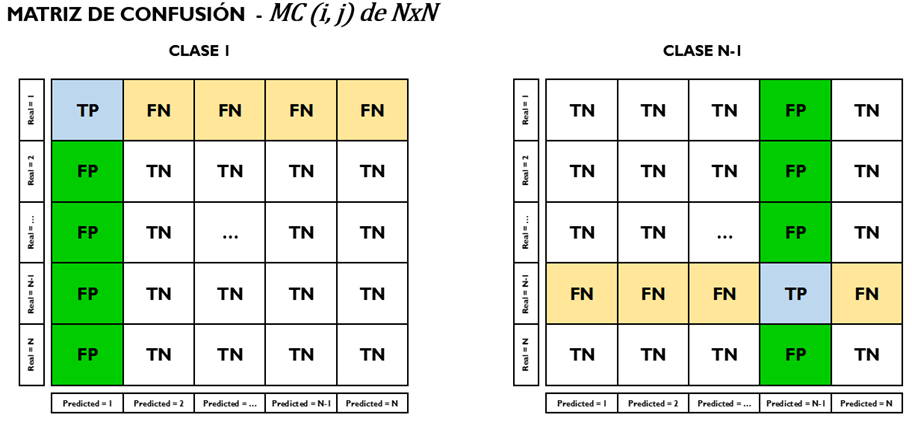
\includegraphics[width=1\textwidth]{./Figures/matriz-confusion.png}
	\caption{Ejemplo de matriz de confusión multiclase genérica\protect\footnotemark.}
	\label{fig:matriz-confusion}
\end{figure}

\footnotetext{Imagen tomada de \url{https://wbarriosb.medium.com/calculando-la-precisi\%C3\%B3n-en-un-modelo-de-clasificaci\%C3\%B3n-multiclase-224d96f52043}}

Para entender esta matriz, es necesario presentar cuatro conceptos que vienen asociados:
\begin{itemize}
	\item Verdaderos positivo (VP o TP): la cantidad de positivos clasificados como positivos por el modelo.
	\item Falso negativo (FN): la cantidad de positivos clasificados como negativos por el modelo.
	\item Verdadero negativo (VN o TN): la cantidad de negativos clasificados como negativos por el modelo.
	\item Falso positivo (FP): la cantidad de negativos clasificados como positivos por el modelo.
\end{itemize}

Presentar los resultados en esta matriz permite calcular distintas métricas para evaluar características del sistema de clasificación. Por ejemplo:

La precisión, que está relacionada con la capacidad del modelo de no predecir un positivo cuando en realidad es un negativo:
\begin{equation}
\text{precisión}_{k}=\frac{MC(k,k)}{\sum_{i=1,j=k}^{N}MC(i,j)}
\end{equation}

La exhaustividad, que está relacionada con la capacidad del modelo de detectar todos los positivos:
\begin{equation}
\text{exhaustividad}_{k}=\frac{MC(k,k)}{\sum_{j=1,i=k}^{N}MC(i,j)}
\end{equation}

Para este trabajo, la métrica seleccionada para evaluar el desempeño de los modelos fue el puntaje F1 o \textit{F1-Score}. Lo que hace esta métrica es calcular la media armónica entre la precisión y la exhaustividad \textit{(recall)} del modelo. Su fórmula es la siguiente:
\begin{equation}
\text{F1}_{k}=2\times \frac{\text{precisión}_{k}\times \text{exhaustividad}_{k}}{\text{precisión}_{k}+ \text{exhaustividad}_{k}}
\end{equation}

De esta forma, se estaría obteniendo el F1 para cada clase. Para calcular un F1 global del sistema de clasificación, existen tres tipos de estrategia \citep{WEBSITE:28}
\begin{itemize}
	\item \textit{Macro average}: Consiste en calcular la media aritmética de todos los F1 calculados para cada clase. Esta estrategia le da a todas las clases la misma importancia en el cálculo del F1 global.
	\item \textit{Micro average}: Consiste en calcular el F1 considerando el número total de TP, FP y FN, en lugar de hacerlo por cada clase. Esta estrategia calcula la proporción de las observaciones clasificadas correctamente sobre las observaciones totales.
	\item \textit{Weighted average}: Consiste en calcular la media aritmética de todos los F1 calculados para cada clase, pero ponderando el soporte de cada clase (la cantidad de observaciones). Esta estrategia le da más importancia a las clases con más observaciones para el cálculo del F1 global.
\end{itemize}

Para \textit{datasets} balanceados, es decir, cuando tienen una cantidad de observaciones parecida para cada una de las clases, se suele usar el \textit{micro average}. No es el caso de este trabajo, donde por la naturaleza de los reclamos, hubo categorías que presentaron más observaciones que otras.

Dentro de las dos opciones restantes, se decidió por utilizar el \textit{weighted} F1, ya que para medir el desempeño del modelo, se pretende dar una mayor importancia a las clases cuyos reclamos aparecen más a menudo. 

La fórmula se muestra a continuación:
\begin{equation}
\text{F1}_{global}=\sum_{k=1}^{N}\text{F1}_{k} \times \text{soporte}_{k} 
\end{equation}

\section{Resultados de desempeño en pruebas}

En esta sección se presentan los resultados obtenidos para todos los modelos entrenados de cada categoría.

\subsection{Resultados para clasificador L1}

En la figura \ref{fig:res-l1} se pueden observar los distintos entrenamientos realizados para el clasificador L1 y su puntaje obtenido:

\begin{figure}[htbp]
	\centering
	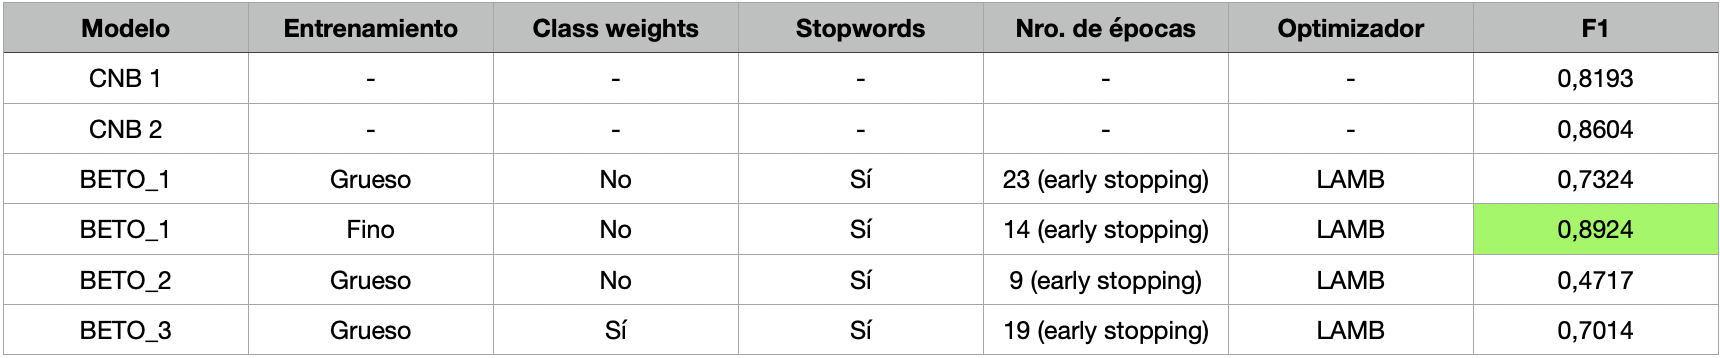
\includegraphics[width=1\textwidth]{./Figures/cap4-resultados-l1.png}
	\caption{Resultados obtenidos para los modelos clasificadores L1.}
	\label{fig:res-l1}
\end{figure}

A continuación se hacen algunas aclaraciones respecto de los modelos:
\begin{itemize}
	\item Modelo CNB\_1: los reclamos pertenecientes a la categoría especial que se menciona en la subsección \ref{sec:extraccion} fueron eliminados.
	\item Modelo CNB\_2: los reclamos pertenecientes a la categoría especial fueron redireccionados a otras categorías L1.
	\item Modelo BETO\_1: los reclamos pertenecientes a la categoría especial fueron eliminados.
	\item Modelo BETO\_2: los reclamos pertenecientes a la categoría especial fueron redireccionados a otras categorías L1.
	\item Modelo BETO\_3: los reclamos pertenecientes a la categoría especial fueron eliminados.
\end{itemize}

\subsection{Resultados para clasificador L2 A}

En la figura \ref{fig:res-l2a} se pueden observar los distintos entrenamientos realizados para el clasificador L2 A y su puntaje obtenido:

\begin{figure}[H]
	\centering
	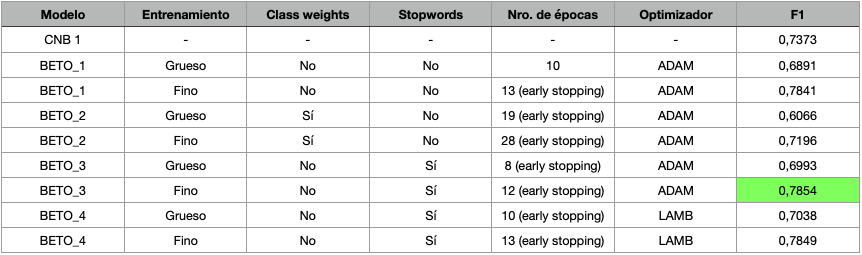
\includegraphics[width=1\textwidth]{./Figures/cap4-resultados-l2a.png}
	\caption{Resultados obtenidos para los modelos clasificadores L2 A.}
	\label{fig:res-l2a}
\end{figure}

Aclaración: el modelo BETO\_4 cuenta con un \textit{head} de clasificación de dos capas.

\subsection{Resultados para clasificador L2 B}

En la figura \ref{fig:res-l2b} se muestran los entrenamientos realizados para el clasificador L2 B y sus resultados:

\begin{figure}[htbp]
	\centering
	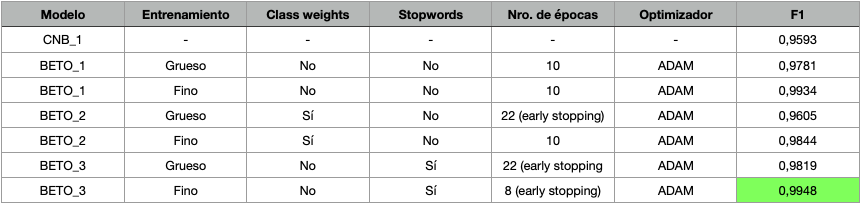
\includegraphics[width=1\textwidth]{./Figures/cap4-resultados-l2b.png}
	\caption{Resultados obtenidos para los modelos clasificadores L2 B.}
	\label{fig:res-l2b}
\end{figure}

\subsection{Resultados para clasificador L2 C}

En la figura \ref{fig:res-l2c} se presentan los resultados para los entrenamientos del clasificador L2 C:

\begin{figure}[htbp]
	\centering
	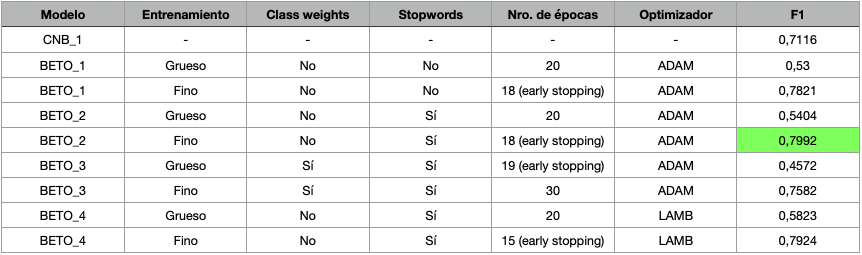
\includegraphics[width=1\textwidth]{./Figures/cap4-resultados-l2c.png}
	\caption{Resultados obtenidos para los modelos clasificadores L2 C.}
	\label{fig:res-l2c}
\end{figure}

Aclaración: los modelos entrenados con LAMB cuentan con un \textit{head} de clasificación de dos capas.

\subsection{Resultados para clasificador L2 D}

A continuación se muestra la figura \ref{fig:res-l2d} con los resultados para los entrenamientos del clasificador L2 D.

\begin{figure}[htbp]
	\centering
	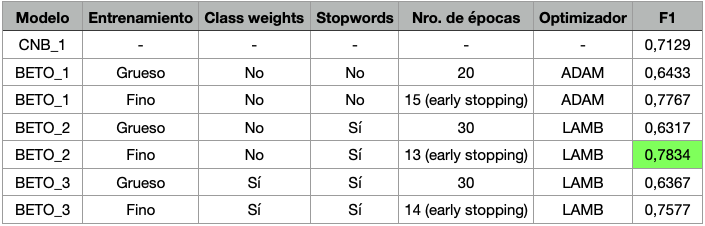
\includegraphics[width=1\textwidth]{./Figures/cap4-resultados-l2d.png}
	\caption{Resultados obtenidos para los modelos clasificadores L2 D.}
	\label{fig:res-l2d}
\end{figure}

Aclaración: los modelos entrenados con LAMB cuentan con un \textit{head} de clasificación de dos capas.

\subsection{Resultados para clasificador L2 E}

En la figura \ref{fig:res-l2e} se pueden observar los distintos entrenamientos realizados para el clasificador L2 E y su puntaje obtenido:

\begin{figure}[htbp]
	\centering
	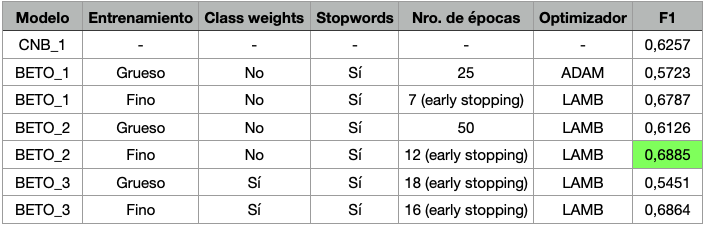
\includegraphics[width=1\textwidth]{./Figures/cap4-resultados-l2e.png}
	\caption{Resultados obtenidos para los modelos clasificadores L2 E.}
	\label{fig:res-l2e}
\end{figure}

A continuación se hacen algunas aclaraciones:
\begin{itemize}
	\item Los modelos CNB\_1 y BETO\_1 fueron entrenados únicamente con el dataset que tenía datos hasta 2022. Algunas categorías no tenían datos hasta esa fecha, por lo que los modelos fueron entrenados con datos faltantes para esas categorías.
	\item Los modelos BETO\_2 y BETO\_3 fueron entrenados con el dataset que tenía datos hasta 2022 pero incluyendo datos de 2023 para las categorías que no tenían datos.
\end{itemize}

\subsection{Resultados para clasificador L2 F}

En la figura \ref{fig:res-l2f} se muestran los entrenamientos realizados para el clasificador L2 F y sus resultados:

\begin{figure}[H]
	\centering
	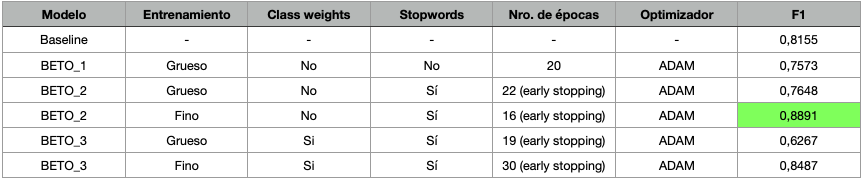
\includegraphics[width=1\textwidth]{./Figures/cap4-resultados-l2f.png}
	\caption{Resultados obtenidos para los modelos clasificadores L2 F.}
	\label{fig:res-l2f}
\end{figure}

\subsection{Resultados para clasificador L2 G}

En la figura \ref{fig:res-l2g} se presentan los resultados para los entrenamientos del clasificador L2 G:

\begin{figure}[htbp]
	\centering
	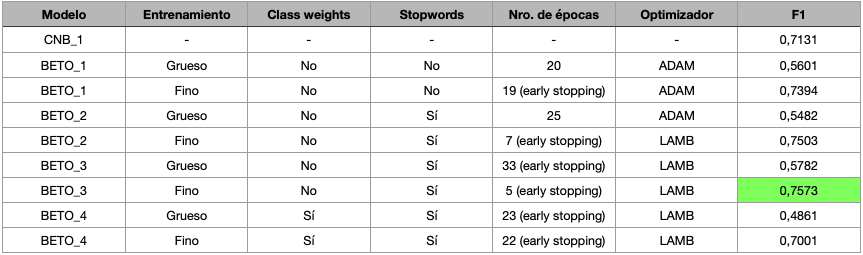
\includegraphics[width=1\textwidth]{./Figures/cap4-resultados-l2g.png}
	\caption{Resultados obtenidos para los modelos clasificadores L2 G.}
	\label{fig:res-l2g}
\end{figure}

Aclaración: los modelos BETO\_3 y BETO\_4 fueron entrenados con un \textit{head} de clasificación de dos capas.

\subsection{Resultados para clasificador L2 H}

A continuación se muestra la figura \ref{fig:res-l2h} con los resultados para los entrenamientos del clasificador L2 H.

\begin{figure}[htbp]
	\centering
	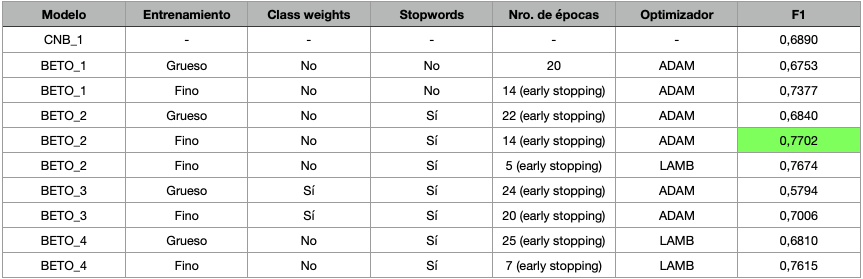
\includegraphics[width=1\textwidth]{./Figures/cap4-resultados-l2h.png}
	\caption{Resultados obtenidos para los modelos clasificadores L2 H.}
	\label{fig:res-l2h}
\end{figure}

Aclaración: el modelo BETO\_4 fue entrenado con un \textit{head} de clasificación de dos capas.

\subsection{Resultados para clasificador L2 I}

En la figura \ref{fig:res-l2i} se presentan los resultados para los entrenamientos del clasificador L2 I.

\begin{figure}[htbp]
	\centering
	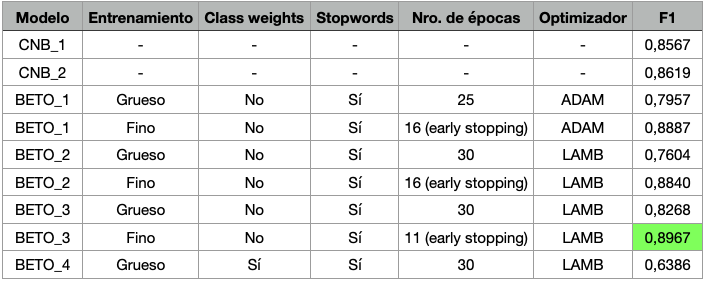
\includegraphics[width=1\textwidth]{./Figures/cap4-resultados-l2i.png}
	\caption{Resultados obtenidos para los modelos clasificadores L2 I.}
	\label{fig:res-l2i}
\end{figure}

Se hacen algunas aclaraciones:
\begin{itemize}
	\item Tanto en el dataset que tenía datos hasta 2022 como el que incluía datos de 2023 carecían de datos para algunas categorías.
	\item Todos los modelos entrenados con LAMB contaban con un \textit{head} de clasificación de dos capas.
	\item El modelo BETO\_1 fue entrenado exclusivamente con el dataset original.
	\item El modelo BETO\_2 fue entrenado con el dataset original y se incluyeron datos de 2023 para las categorías sin datos.
	\item Los modelos BETO\_3 y BETO\_4 fueron entrenados con datos hasta 2023 inclusive para todas las categorías.
\end{itemize}

\subsection{Resultados para clasificador L2 J}

A continuación se muestra la figura \ref{fig:res-l2j} con los resultados para los entrenamientos del clasificador L2 J.

\begin{figure}[htbp]
	\centering
	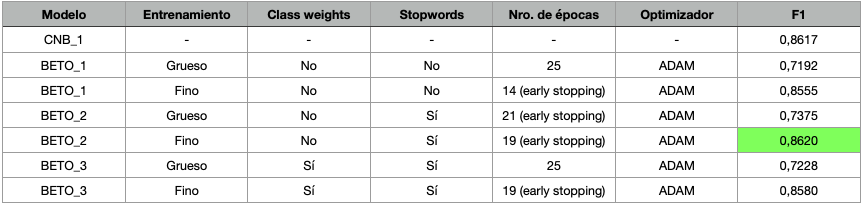
\includegraphics[width=1\textwidth]{./Figures/cap4-resultados-l2j.png}
	\caption{Resultados obtenidos para los modelos clasificadores L2 J.}
	\label{fig:res-l2j}
\end{figure}

\subsection{Resultados para clasificador L2 K}

En la figura \ref{fig:res-l2k} se presentan los resultados para los entrenamientos del clasificador L2 K.

\begin{figure}[htbp]
	\centering
	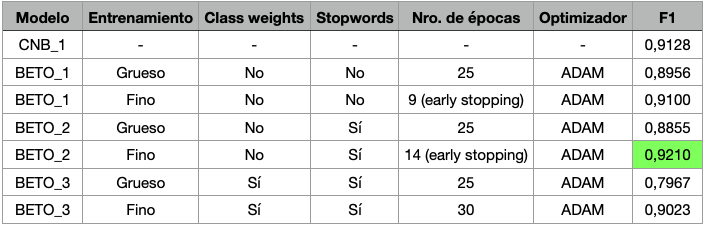
\includegraphics[width=1\textwidth]{./Figures/cap4-resultados-l2k.png}
	\caption{Resultados obtenidos para los modelos clasificadores L2 K.}
	\label{fig:res-l2k}
\end{figure}

\subsection{Resultados para clasificador L2 L}

En la figura \ref{fig:res-l2l} se presentan los resultados para los entrenamientos del clasificador L2 L.

\begin{figure}[htbp]
	\centering
	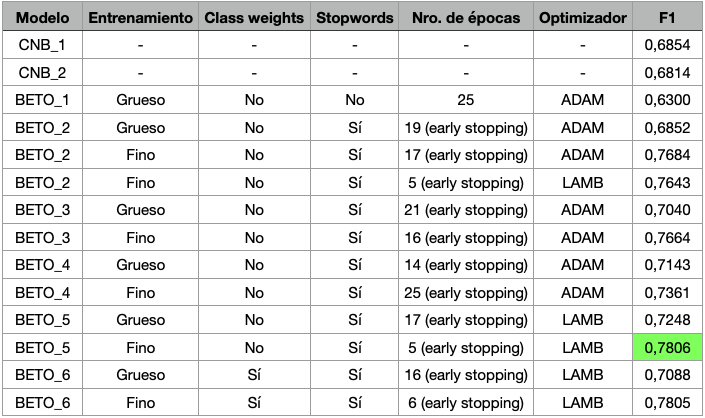
\includegraphics[width=1\textwidth]{./Figures/cap4-resultados-l2l.png}
	\caption{Resultados obtenidos para los modelos clasificadores L2 L.}
	\label{fig:res-l2l}
\end{figure}

Se hacen algunas aclaraciones de los modelos:
\begin{itemize}
	\item Los modelos CNB\_1, BETO\_1 y BETO\_2 fueron entrenados con el dataset original que tenía datos hasta 2022 inclusive.
	\item Los modelos CNB\_2, BETO\_3, BETO\_5 y BETO\_6 fueron entrenados con el dataset que también incluía datos de 2023.
	\item Para el entrenamiento del modelo BETO\_4 se utilizó el dataset original que tenía datos hasta 2022 y además se incluyeron datos de 2023 para la clase minoritaria.
	\item Para los modelos BETO\_5 y BETO\_6 se utilizó un \textit{head} de clasificación de dos capas.
\end{itemize}

\subsection{Resultados para clasificador L2 M}

Como se mencionó en la sección \ref{sec:kfolds}, el entrenamiento del modelo L2 M fue particular porque se contaban con 267 muestras incluyendo los casos de 2023. Se decidió obtener una métrica con validación cruzada para tener una medida de desempeño y luego entrenar un modelo con todos los datos. En este caso el F1 obtenido fue 0,5568.

\subsection{Resultados para clasificador L2 N}

Además, en la sección \ref{sec:kfolds} también se hace mención al modelo L2 N, que fue un caso extremo donde sólo había 8 muestras incluyendo los datos de 2023. Aquí se utilizó la técnica de \textit{leave one out} y el F1 obtenido fue 0,7500.

\section{Simulación en ambiente de desarrollo}


